% 2015-10-01 - Matthew A. Wolff - Thesis research presentation

\documentclass{beamer}

\mode<presentation> {
	% Themes and color schemes:
	\usetheme{default}
	\usecolortheme{rose}
}

% Need this on campus machine (but not at home)
\usepackage{sansmathaccent}
\pdfmapfile{+sansmathaccent.map}

\usepackage{graphicx} % Allows including images
\usepackage{booktabs} % Allows the use of \toprule, \midrule and \bottomrule in tables
\usepackage{mathtools} % Allows to declare paired delimiters

\DeclarePairedDelimiter\ceil{\lceil}{\rceil}
\DeclarePairedDelimiter\floor{\lfloor}{\rfloor}

%------------------------------------------------------------------------------
%	TITLE PAGE
%------------------------------------------------------------------------------

% The short title appears at the bottom of every slide, the full title is only on the title page
\title[Multilevel Summation Method]{Multilevel Summation Method} 

\author{Matthew A. Wolff} % Your name
\institute[Purdue University] % Your institution as it will appear on the bottom of every slide, may be shorthand to save space
{
	Purdue University \\ % Your institution for the title page
	\medskip
	\textit{wolff1@purdue.edu} % Your email address
}
\date{October 1, 2015} % Could also use \today, if desired

% Add slide numbers
\setbeamerfont{page number in head/foot}{size=\small}
\setbeamertemplate{footline}[frame number]

\begin{document}

\begin{frame}
	\titlepage % Print the title page as the first slide
\end{frame}

\begin{frame}
	\frametitle{Overview} % Table of contents slide, comment this block out to remove it
	\tableofcontents % Throughout your presentation, if you choose to use \section{} and \subsection{} commands, these will automatically be printed on this slide as an overview of your presentation
\end{frame}

%\section{Timeline}
%
%\frame{
	%\frametitle{Timeline}
%
	%\tiny{
		%\begin{itemize}
			%\item 8/27 - Last presentation (I think)
			%\item 8/31 - Softening function experimentation
			%\item 9/3 - Discussed 1D interpolation errors and moving to 6D
			%\item 9/7 - Read Reimer about spline interpolation error on equidistant grids
			%\item 9/11 - Revamped FMM Cilk code
			%\item 9/14 - Read Richards about Lebesgue constant for cardinal spline interpolation
			%\item 9/14 - Wrote MATLAB code to determine $h$ for given $p$ and $\tau$
			%\item 9/15 - Choosing $k$ based on $p$ for quasi-interpolation
			%\item 9/18 - Decided that $a$ should be defined before $h, p, k,$ etc
			%\item 9/22 - Worked on how to determine $a$
			%\item 9/24 - Read about clustering, k-NN algorithms, etc
			%\item 9/29 - Worked on strategy for computing "optimal" $a$
			%\item 9/30 - More work on "optimal" $a$ and space-filling curves
			%\item 10/2 - Coded prototype for "optimal" $a$
		%\end{itemize}
	%}
%}

\section{Error Analysis}

\frame{
	\frametitle{Error Analysis}
	Goal is to use predicted error to help choose parameters. \\
	Reimer gives cardinal spline interpolation error:
	$$\|f-\tilde{f}\| \leq \left( \frac{h}{2} \right)^p \left( \frac{(1)(3)(...)(p-1)}{(2)(4)(...)(p)} + \| \mathcal{L}^{p-1} \| \right) \|f^{(p)}\| $$
	Richards provides the Lebesgue constant:
	$$\|\mathcal{L}^{p-1}\| = \frac{2}{\pi} \left( \log{(p-1)} + 2 \log{\frac{4}{\pi}} + \gamma \right) + o(1)$$
	where $p-1$ is the degree of the interpolant, $h$ is the spacing between interpolation nodes, and $\gamma$ is the Euler-Mascheroni constant.\\

	Questions:
	\begin{itemize}
		\item Where does the constant term come from? (Integration?)
		\item Why do we have $O(\frac{1}{p})$ instead of $o(1)$?
		\item How should we deal with it? (if we need to at all)
	\end{itemize}
}

\section{Parameter Selection}

\frame{
	\frametitle{Parameter Selection}
	Given $N$ particles and desired error tolerance, $\tau$, MSM needs the following parameters:
	\begin{itemize}
		\item $a$ - cut-off distance
		\item $h$ - grid spacing on finest grid
		\item $p$ - order of interpolation
		\item $k$ - degree of continuity for softening function
%		\item $\mu$ - parameter which controls B-spline coefficient accuracy
	\end{itemize}
}

\subsection{Parameter Selection (Long-range)}

\frame{
	\frametitle{Parameter Selection (Long-range)}
	Long range error has the form:
	\tiny{
	$$\|f-\tilde{f}\| \leq \left( \frac{h}{2} \right)^p \left( \frac{(1)(3)(...)(p-1)}{(2)(4)(...)(p)} + (\frac{2}{\pi} \left( \log{(p-1)} + 2 \log{\frac{4}{\pi}} + \gamma \right) + o(1)) \right) \|f^{(p)}\| $$
	}
	\small
	Taking into account that
	$$f = \frac{1}{a} \bar{\gamma}(r/a)$$
	and
	$$f^{(p)} = \frac{1}{a^{(p+1)}}\bar{\gamma}^{(p)}(r/a)$$
	where $\bar{\gamma}(s)$ is the softening function of degree $2k$, we have:
	\tiny{
	$$\|f-\tilde{f}\| \leq \frac{1}{a^{p+1}}\left( \frac{h}{2} \right)^p \left( \frac{(1)(3)(...)(p-1)}{(2)(4)(...)(p)} + (\frac{2}{\pi} \left( \log{(p-1)} + 2 \log{\frac{4}{\pi}} + \gamma \right) + o(1)) \right) \|\bar{\gamma}^{(p)}\| \leq \tau $$
	}
	\small

	Need to choose $h,p$ such that
	\begin{itemize}
		\item h is as large as possible
		\item p is as low as possible
		\item finest grid, $\Omega^{(1)}$, has $M = O(N)$ grid points
	\end{itemize}
}

\frame{
	\frametitle{Parameter Selection (Long-Range), cont.}
	For interpolation error and specified error tolerance, we need:
	\tiny{
	$$\frac{1}{a^{p+1}}\left( \frac{h}{2} \right)^p \left( \frac{(1)(3)(...)(p-1)}{(2)(4)(...)(p)} + (\frac{2}{\pi} \left( \log{(p-1)} + 2 \log{\frac{4}{\pi}} + \gamma \right) + o(1)) \right) \|\bar{\gamma}^{(p)}\| \leq \tau $$
	}
	\small
	Rearrange terms and solve for $h$ in terms of $p$:
	\tiny
	$$h \leq 2 \sqrt[p]{\frac{a^{(p+1)}\tau}{\left( \frac{(1)(3)(...)(p-1)}{(2)(4)(...)(p)} + (\frac{2}{\pi} \left( \log{(p-1)} + 2 \log{\frac{4}{\pi}} + \gamma \right) + o(1)) \right)\|\bar{\gamma}^{(p)}\|}}$$
	\small
	Note:
	\begin{itemize}
		\item $\|\bar{\gamma}^{(p)}\|_{\infty} \approx \bar{\gamma}^{(p)}(0)$
		\item "messy" constants can be precomputed
		\item A large value of $a$ effectively "raises" tolerance
	\end{itemize}
}

\frame{
	\frametitle{Algorithm}
	\begin{itemize}
		\item p = 2
		\item a = (some known value)
		\item do
			\begin{itemize}
				\item p += 2
				\item k = p/2 - 1
				\item Build $\bar{\gamma}(s)$ with new $k$
				\item Solve:\tiny
	$$h = \floor*{2 \sqrt[p]{\frac{a^{(p+1)}\tau}{\left( \frac{(1)(3)(...)(p-1)}{(2)(4)(...)(p)} + (\frac{2}{\pi} \left( \log{(p-1)} + 2 \log{\frac{4}{\pi}} + \gamma \right) + o(1)) \right)\|\bar{\gamma}^{(p)}\|}}}$$ \small
			\end{itemize}
		\item while $(D/h > M)$
	\end{itemize}
	where $D$ is the domain size and $M = O(N)$ is the number of finest grid points. \\
	Note: 	Added pre-processing cost should be negligible.
}

\subsection{Parameter Selection (Short-range)}

\frame{
	\frametitle{Parameter Selection (Short-range)}
	Error is not a concern in the short-range calculation. Should focus on computational cost instead.\\
	Choose $a$ such that
	\begin{itemize}
		\item $1.0 \leq a \leq D$, where $D$ is the domain size
		\item $a$ is as large as possible
		\item Bins with side-length $a$ contain no more than $\floor*{\sqrt{N}}$ particles
		\item Maximal $a$ improves performance (less overhead looping over bins)
	\end{itemize}
}

\frame{
	\frametitle{Algorithm}
	Define:
	\begin{itemize}
		\item $q := \floor*{\sqrt{N}}$
		\item $r_{k(i)}$ is $q$-th nearest neighbor to $r_i$
		\item $Q(r_i) := \{r_j \in \mathbb{R}^d \text{s.t.} \|r_i - r_j\| \leq \|r_i-r_{k(i)}\|, 1 \leq i,j \leq N\}$ 
		\item $Q(r_i)$ is the set of $q$ nearest neighbors to $r_i$, including $r_i$
	\end{itemize}

	Algorithm:
	\begin{itemize}
		\item $a = D$
		\item For each particle, $r_i, 1 \leq i \leq N$:
		\begin{itemize}
			\item Compute $Q(r_i)$
			\item Sort $Q(r_i)$ such that distances from $r_i$ are in ascending order
			\item $r_{k(i)}$ lies at corner of bin centered at $r_i$ containing $q$ particles
			\item $a = \min{(a, \sqrt{\frac{4}{d}}\|r_i - r_{k(i)}\|)}$
		\end{itemize}
		\item $a = \max{(a, 1.0)}$
	\end{itemize}
}

\frame{
	\frametitle{Short-range visualization - 1}
	\begin{center}
		\mbox{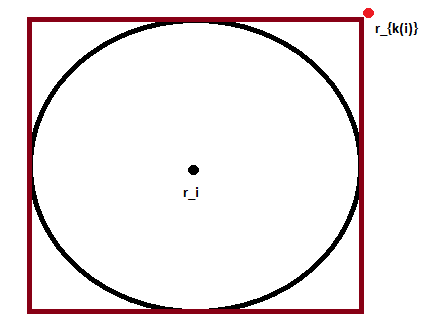
\includegraphics[width=0.9 \textwidth]{../Figures/BoundingBox1.png}}
	\end{center}
}

\frame{
	\frametitle{Short-range visualization - 2}
	\begin{center}
		\mbox{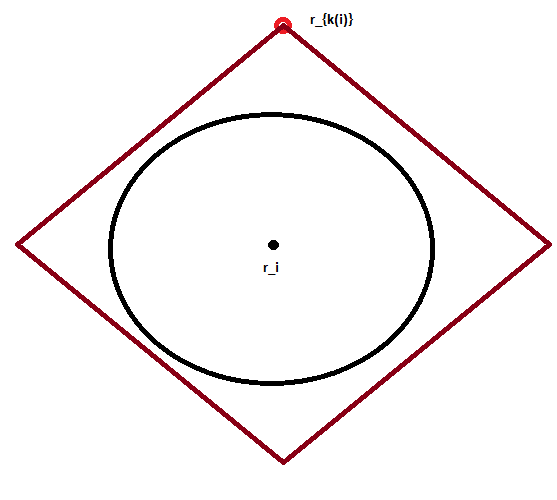
\includegraphics[width=0.9 \textwidth]{../Figures/BoundingBox2.png}}
	\end{center}
}

\frame{
	\frametitle{Additional short-range thoughts}
	Current algorithm is naive ($O(N^2 \log{N})$).\\
	I believe space-filling curve combined with bucket sorting would allow for $O(N)$ complexity. (This claim supported, I think, by German thesis in related field.)
}

\frame{
	\frametitle{The End!}
	\begin{center}
		Thank you!
	\end{center}
}

\end{document}